\chapter{Power Plant Cost Model Preparation}\label{ch4:cm_prep}

\section{EGS Expansion Concept}\label{ch4:cm_concept}
\subsection{Lightning Dock EGS}

Lightning Dock (Section \ref{ch2:lightning_dock}) is presently the only commercial power plant operating in the state of New Mexico. The net generating capacity after its first phase of development was 4 MW in 2013, with the expectation of upgrading to 10 MW in a second development phase that never came to fruition. Instead, the facility underwent a significant refit in 2018, resulting in a net capacity of 11.2 MW generated entirely from hydrothermal brine production \citep{bonafin_repowering_2019}. 

Department of Energy-funded efforts to characterize the geothermal resources in the Animas Valley, NM revealed the presence of two different thermal reservoirs: the hydrothermal resource targeted by Lightning Dock where deep geothermal fluids ascend along the Animas Valley Fault complex to $\approx$365-1000 m depth, and a secondary interval at $\approx$900-1200 m depth that requires permeability enhancement for production \citep{schochet_development_2001}. The Horquilla limestone formation defines the second reservoir, estimated to span a minimum volume of 6 cubic km based on conservative figures. By one proprietary study completed in 2001 for Ormat Technologies, a commercial geothermal company, the Horquilla has a 88\% probability of 6 MW in recoverable electricity generation potential \citep{schochet_development_2001}.

\citet{schochet_development_2001} proposed the construction of a 6 MW hybrid power plant combining hydrothermal and EGS-sourced power generation a decade before operations commenced at Lightning Dock. In their development plan, they noted several benefits of pursuing EGS in this location:
\begin{itemize}[itemsep=2pt]\label{ch4:ld_egs_support}
    \item Relatively shallow resource drives lower drilling costs
    \item EGS water requirements are attainable from paired hydrothermal operations
    \item A comprehensive initial assessment determined no significant environmental degradation is expected from geothermal operations
    \item Lightning Dock has direct access to in-place transmission lines  
    \item Opportunities exist for electricity sales to local users
    \item Purchase agreements with regional utilities are incentivized by NM legislation
\end{itemize}

As suggested by this list, the conditions at Lightning Dock offer a nearly ideal test case for an EGS proof of concept on a manageable scale. Historical land utilization in the area is primarily agricultural with few residences, so risk is low for any adverse impact on an existing population. In addition, use of a binary cycle design as proposed by \citet{schochet_development_2001} offers the potential for power production with zero GHG emissions.  

In this thesis, the \citeauthor{schochet_development_2001} concept is revisited with the existing geothermal production at Lightning Dock kept in mind; rather than building a new hybrid facility, the revised concept involves targeting the deeper reservoir as a near-hydrothermal field EGS (NF-EGS) development with a tie-back to the current Lightning Dock facility. Stepping out from the hydrothermal zone in proximity to the Animas Valley Fault complex, thermal conditions settle to a high background geothermal gradient between $\approx$ 80-120 K/km based on boreholes TG 56-14 and TG 12-7 \citep{cunniff_final_2003} -- certainly high enough to support geothermal capture. These conditions make for an interesting case study on risk mitigation options for EGS production planning.

Public records regarding power generation at Lightning Dock provide some guidance on the appropriate size for an EGS expansion. After phase 1 development, the plant produced 4 MW. An additional 6 MW was slated for phase 2, but re-powering of the plant actually added 7 MW to the capacity after several years of development stasis \citep{think_geoenergy_turboden_2020}. \citeauthor{schochet_development_2001} originally proposed a 6 MW hybrid plant for the site, but they also noted 6 MW from the Horquilla was likely understating the full reservoir potential \citeyear{schochet_development_2001}. In consideration of the step-wise trajectory of plant improvements and assessment of available thermal resource, this case study targets 5 MW as a expansion goal. 

\subsection{New Mexico Electricity Demand}

Pursuing the expansion of a power plant requires sufficient demand to ensure total revenue offsets project expenses. Fortunately, New Mexico regulations support the further development of geothermal power production in the state. Specifically, the Energy Transition Act signed in 2019 updated the New Mexico \acrlong{rps} (\acrshort{rps}) to go zero-carbon by 2050, with milestone targets along the way \citep{lillian_new_2019}. The RPS dates back to the Renewable Energy Act passed in 2004 and comes with several carve-outs, including a 30\% requirement for wind energy, 20\% for solar, and 5\% for other renewables like geothermal \citep{dsire_dsire_2021}. Public Service Company of New Mexico (PNM) is the state’s largest energy provider and services the Lordsburg area where Lightning Dock is located. PNM and Cyrq Energy currently share a 20-year \acrlong{ppa} (\acrshort{ppa}) for electricity generated at Lightning Dock. The PPA has gone through amendments over time to update both the wattage supplied to PNM and the pricing structure per MWh \citep[e.g.,][]{pnm_pnm_2014,stanfield_new_2017}. This indicates a PPA can be revisited if conditions change, which is an important aspect to consider when modeling project financials. 
In addition to the RPS requirement for a diversified renewables portfolio, coal power plants across the state face mandated shut-downs as a consequence off the Energy Transition Act. Coal currently supplies a large fraction ($\approx$ 45\%) of electric power sector consumption in New Mexico (Figure \ref{fig:nm_energy_consumption}). The supply gap introduced as coal-based production ramps down to zero could more than compensate for a 5 MW addition of no-emissions energy to the New Mexico grid.

\begin{figure}[!htp]
\centering
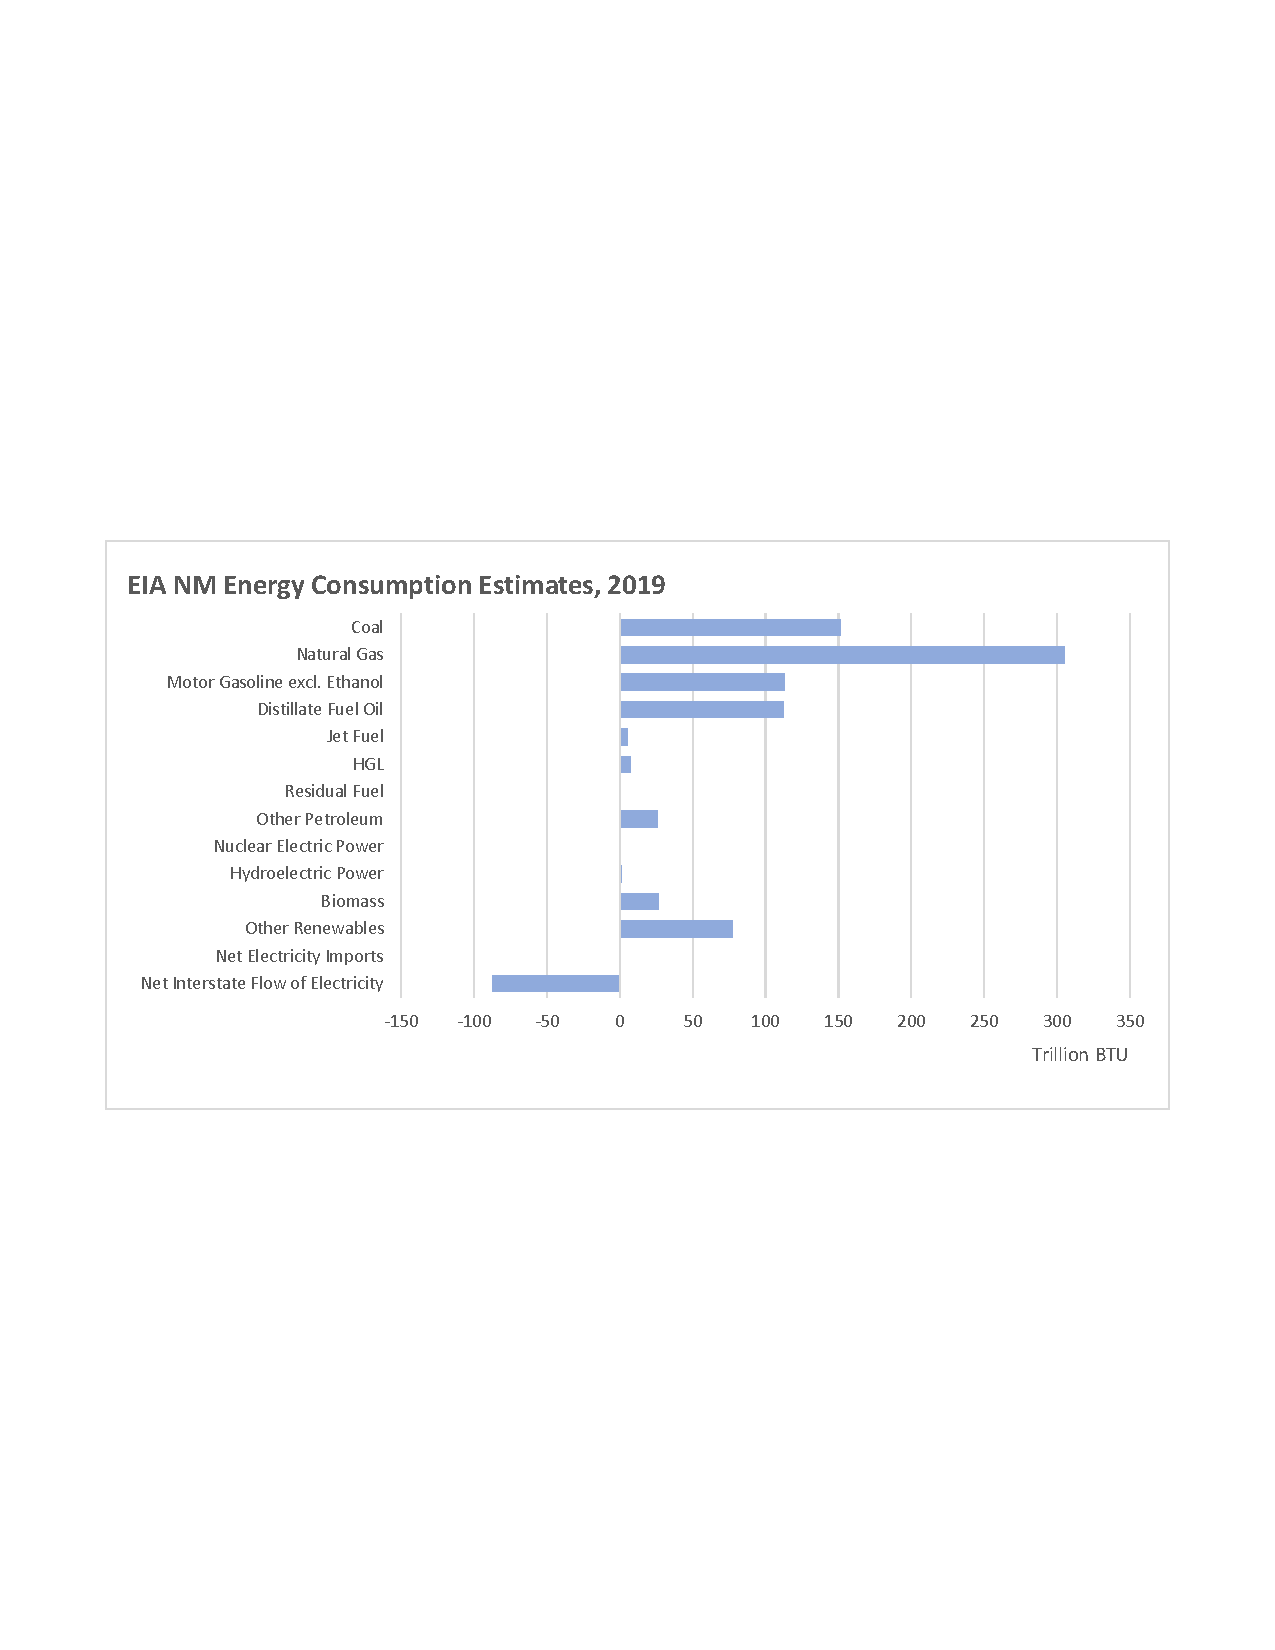
\includegraphics[width=\textwidth]{templates/images/Figure-EIA_NM_Energy_Consumption.pdf}
\caption[NM energy consumption]{Energy consumption by source for New Mexico. Adapted from data and graphics reported by the EIA \protect\citep{eia_new_2021}.}
\label{fig:nm_energy_consumption}
\end{figure}

\subsection{Modular Geothermal}
Limiting this expansion to a single 5 MW facility represents one design alternative, but others exist as well. One flexible option uses modular technology that recently captured the attention of high-stakes investors across the world \citep{shieber_bill_2019}. Climeon has engineered a compact binary cycle unit capable of 150 kW of generated electricity using inlet fluid temperatures rated up to 120℃ and flow rates of up to 35 kg/s \citep{climeon_climeon_2021-1}. These units can be combined into a larger deployable Power Block for 1050 kW of generated electricity \citep{winther_power_2018} (Figure \ref{fig:climeon_powerblock}). Using this technology, power plants can now be treated like multi-unit assemblages, installed all at once or over an extended period of time based on operator needs \citep{climeon_why_2018}.

\begin{figure}[!htp]
\centering
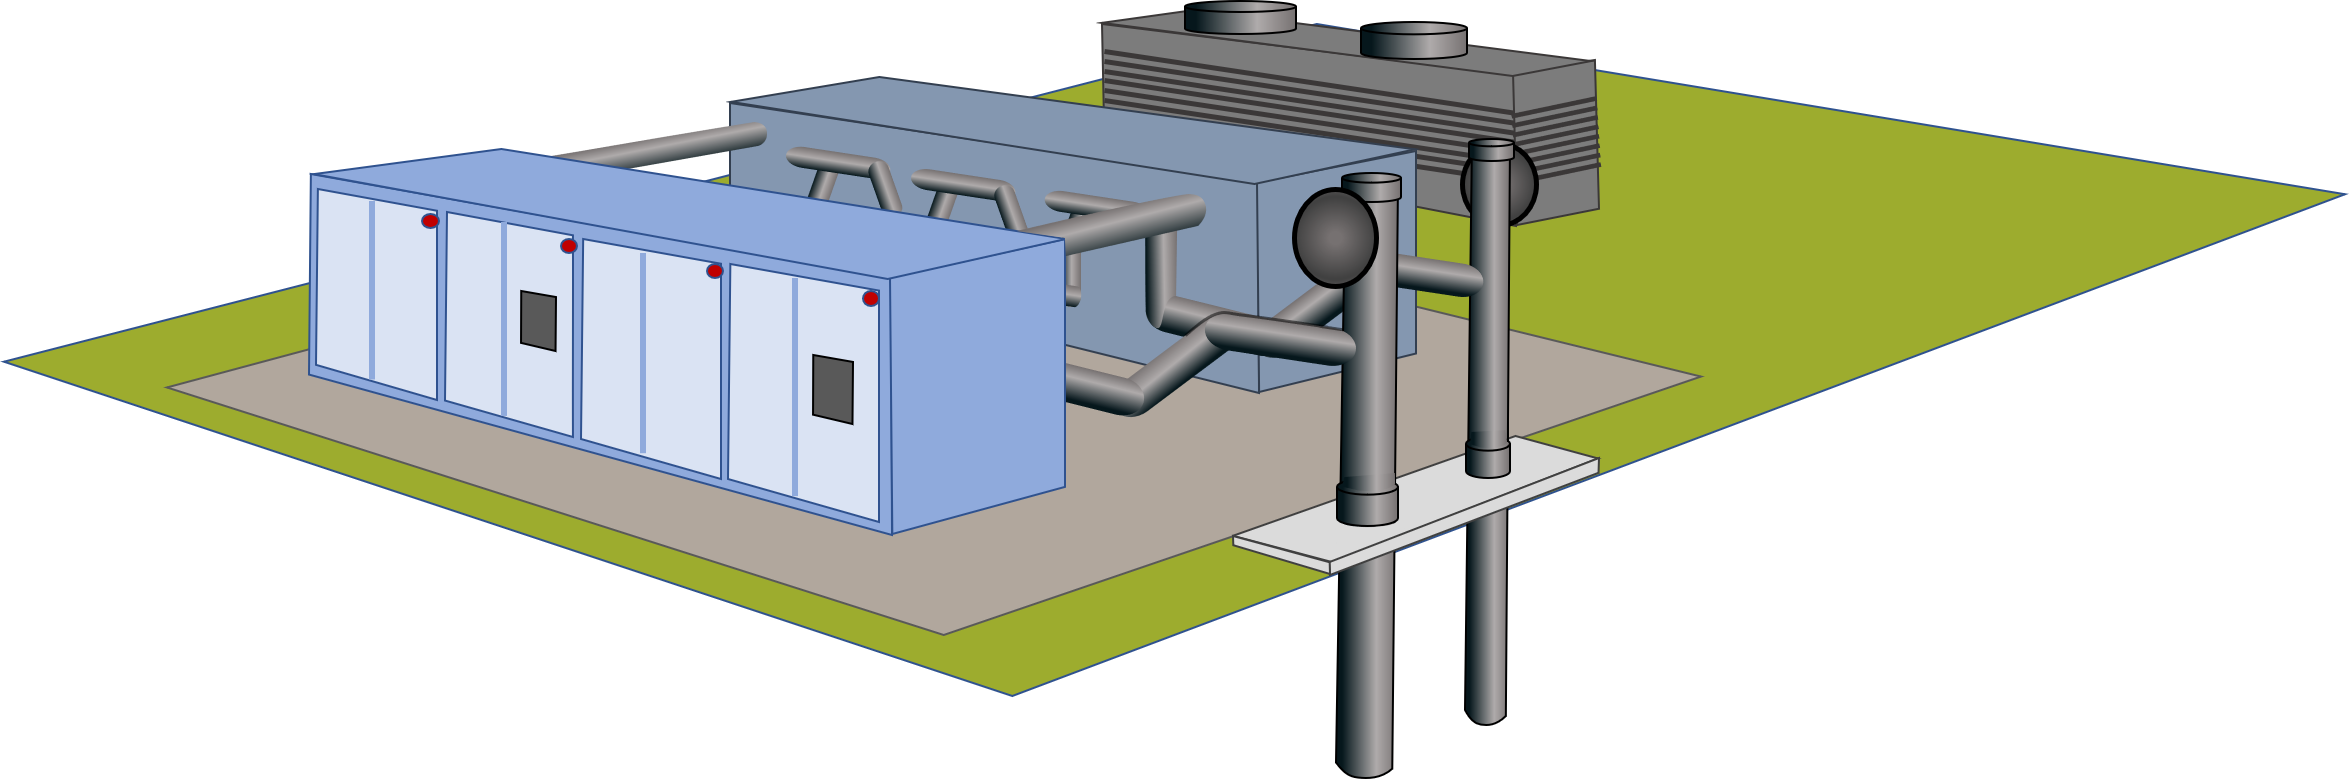
\includegraphics[width=\textwidth]{templates/images/Figure-Climeon-PowerBlock.png}
\caption[Modular power plant schematic]{Modular binary cycle power plant concept, adapted from Climeon PowerBlock schematic diagram \protect\citep{climeon_climeon_2021-1}. Each block consists of seven active units chained together for $\approx$1 MW of generating capacity.}
\label{fig:climeon_powerblock}
\end{figure}

\subsection{Flexibility with Real Options}
As discussed in Section \ref{ch2:costmod}, cost models can provide insights into the potential value gained or lost by a proposed facility before construction even begins. Well-established geothermal cost models like GETEM \citep{entingh_volume_2006} present a highly parameterized but deterministic view of cost and investment opportunity given a defined geothermal resource and development concept. Other models may apply different assumptions or mathematical treatments for various facets of the system, however they uniformly offer a single-track aspect to how the project unfolds over its lifecycle. Users can test ideas, but the solution space remains under-explored due to implicit assumptions of variable trends or static behaviors for a highly-dynamic system.  

In the cost model outlined below, the economic analysis incorporates uncertainty by replacing single value estimates with distributions for model variables. This enables the model to produce a representative range of possible outcomes when simulated many times over. In addition, the model flexibly adapts by executing real (engineering) options, where design updates triggered by changing conditions allow the system to realize upside potential or characterize the extent of downside risk. Designs need not be static, and real options can greatly increase the expected value of a project by exploring execution strategies otherwise missed by more traditional modeling approaches \citep[chap.6]{de_neufville_flexibility_2011}.

\section{Cost Model Structure}
\label{ch4:cm_structure}

Geothermal cost models typically report Levelized Cost of Electricity (LCOE) for simple comparison with other renewable energy sources. However, LCOE is standardized to represent the total lifetime costs incurred by a power plant normalized by the total lifetime power generation from start-up to plant decommissioning. LCOE is therefore not well-suited for communicating projected gains or losses under different designs or scenarios, which are the focus of this analysis. Instead, the model described here relies on \acrlong{npv} (\acrshort{npv}), a simple measure of project lifetime worth that accounts for the time value of money by applying a single interest rate, the discount rate, for both borrowing and deposits \citep[p.\ 195-215]{de_neufville_flexibility_2011}. Here, "present value" refers to a 2020 cost basis. For power generation over a 30-year lifespan -- the default for geothermal models like GETEM \citep{entingh_volume_2006} -- this basis takes the model out to 2050, a common benchmark year for future projections. 

\subsubsection{NPV Model}
\label{ch4:cm_npv}
Following the general outline for geothermal cost modeling from different sources \citep[e.g.,][]{augustine_hydrothermal_2009, beckers_introducing_2013,tester_future_2006}, this thesis considers revenue (R), operating and maintenance costs (OM), and capital expenditures (C) as the primary cash flow elements with a time dependency related to the constant discount rate (r). Capital expenses can be further decomposed into five sub-components associated with exploration, drilling \& completions, reservoir stimulation, fluid distribution, and power plant costs (Equation \ref{eq:cm_components}).

\begin{equation}
    \label{eq:cm_components}
    \begin{aligned}
    NPV &= \sum_{t=1}^{T}\frac{R_t - OM_t - C_t}{(1+r)^t}\\
    \text{where:}\\
    C_t &= \left[C_{expl} + C_{dc} + C_{stim} + C_{dist} + C_{pp}\right]_t
     \end{aligned}
\end{equation}
\\
Revenue and expenses are treated on an annual basis, meaning shorter-term fluctuations like price and production seasonality are not explicitly modeled.

\subsubsection{Exploration Costs} \label{ch4:cm_capex_expl}
Costs for exploration activities are estimated by the same method defined for the 2012 GETEM model (Equation \ref{eq:cm_cexpl}) \citep{eere_getem_2012}. 

\begin{equation}
\label{eq:cm_cexpl}
    C_{expl} = PI \cdot \left[ 1.12 \cdot (\$1\text{M} + 0.6\cdot C_{stdwell}) \right]
\end{equation}
\\
This relationship assumes slim hole (3-6" diameter) drilling for exploration at a 60\% discounted cost compared to standard-sized ($\geq$ 8.5" diameter) geothermal wells. The constant \$1M term accounts for pre-drilling costs, including field work, geophysical surveys of field structure, and interpretation of results. Technical and office support is covered by an additional 12\% applied to the estimate \citep{eere_getem_2012}. Total exploration costs are converted to a 2020 cost basis using the producer price index (PI) for electric power generation from the U.S. Bureau of Labor and Statistics \citep{us_bls_ppi_2021}.

\subsubsection{Drilling \& Completions Costs} 
\label{ch4:cm_capex_dc}

Geothermal drilling and completions costs differ from traditional oil \& gas wells due to differences in hole diameter, thermal and geochemical conditions, and the strength and abrasiveness of the target formations \citep{lowry_geovision_2017}. Here, capital expenditures for drilling rely on the cost curve described by \citet{beckers_introducing_2013}.

\begin{equation}
\label{eq:cm_cdc}
    C_{dc} = PI \cdot \left[ 1.65 \cdot 10^{-5} \cdot MD^{1.607} \right]
\end{equation}
\\
where $C_{dc}$ is measured in \$M and MD refers to well measured depth in meters. Each power plant module will require an injector-producer pair, so this represents one-half of the drilling cost per module. Drilling costs are converted to a 2020 cost basis using the industry index for electric power generation \citep{us_bls_ppi_2021}. 

Note that Equation \ref{eq:cm_cdc} was derived for well depths of 1600-9000 m. Assuming an average geothermal gradient of 100 K/km (Table \ref{tab:cm_resource_params}), the wells considered for this study could extend slightly shallower than this range, so this should be viewed as a minimum drilling \& completions estimate. The stochastic model considered later in this study includes variability in both geothermal gradient and drilling costs for a more comprehensive treatment of both variables.

\subsubsection{Simulation Costs}
\label{ch4:cm_stim}

EGS at Lightning Dock requires stimulation of the Horquilla reservoir to create fluid pathways for thermal extraction. The stimulation cost estimate used in this study comes from the recent GeoVision analysis \citep{lowry_geovision_2017}:

\begin{equation}
\label{eq:cm_capex_stim}
    C_{stim} = \$1,250,000
\end{equation}
\\
Since this represents a recent ballpark estimate, no cost basis conversion was applied in the model. In fact, the value in Equation \ref{eq:cm_stim} may be high since it includes the cost of water, which may not be a factor at Lightning Dock with the availability of hydrothermal brine from adjacent power plant operations. The model assumes stimulation is only performed for the injection well in each injector-producer pair, so this represents a \textit{per module} value.

\subsubsection{Distribution Costs}
\label{ch4:cm_capex_dist}

Fluid distribution costs include the entire surface piping system between the wells and power plant modules. This study uses the same estimate included in the GEOPHIRES model \citep{beckers_introducing_2013}.

\begin{equation}
\label{eq:cm_dist}
    C_{dist} = \$50,000 \cdot q
\end{equation}
\\
where $q$ is the thermal power of the produced geofluid in MW. Under the scenario where modular power plant units are provided by a company like Climeon, fluid distribution may be included in the installation fees. Distribution capital expenditures would therefore be subsumed by power plant costs and $C_{dist}$ would reduce to zero. However, without confirmation of the fee break-down structure from Climeon, the model described here relies on Equation \ref{eq:cm_dist}. 

\subsubsection{Power Plant Costs}
\label{ch4:cm_capex_pp}

Power plant costs for a modular installation remain a source of significant uncertainty for this cost model. The GEOPHIRES model implements a temperature-variable cost estimate first described by \citet{tester_future_2006} for a binary cycle power plant \citep{beckers_introducing_2013}. \citet{schochet_development_2001} predicted produced fluid temperatures of 280-320$^\circ$F (137-160 $^\circ$C) for the Lightning Dock EGS reservoir, which equates to \$1565-\$1694 per kWh by the GEOPHIRES estimate. Converted to a 2020 cost basis \citep{us_bls_ppi_2021}, this amounts to \$2230-\$2415 per kWh.

If power plant capacity is modularized with pre-fabricated units like the Climeon PowerBlock concept, economies of scale should reduce the cost of construction and installation. Unanswered company inquiries left this rationale unconfirmed. Nevertheless, the author chose to assume a round-number estimate accounting for a modularity discount (Equation \ref{eq:cm_pp}). This could easily be replaced by more accurate numbers when those values become available.

\begin{equation}
\label{eq:cm_pp}
    C_{pp} = \$2,000 \cdot q
\end{equation}
\\
The value in Equation \ref{eq:cm_pp} represents a 2020 estimate. Pump costs are assumed to be included in this expense.

\subsubsection{Operations and Maintenance Expenses}
\label{ch4:cm_opex}

Operations and Maintenance expenditures can similarly be subdivided into subsidiary costs, including those related to the power plant, wells, and water management \citep{beckers_introducing_2013}.

\begin{equation}
    \label{eq:cm_opex}
    OM_t = \left[C_{OM,pp} + C_{OM,well} + C_{OM,water}\right]_t
\end{equation}


\subsubsection{Model Parameters}
In order to estimate the values of these components, the following parameters were defined for a deterministic cost model. The values selected are reflective of the Animas, NM region, the Lightning Dock facility, and limits on components of the system to the best of the author's knowledge.
\\
\\
The following parameters relate to resource recovery:
\begin{table}[!htp]
\centering
\resizebox{\textwidth}{!}{
\begin{tabular}{|l|c|l|}
\hline
\multicolumn{1}{|c|}{\textbf{Parameter}} & \textbf{Value} & \multicolumn{1}{c|}{\textbf{Reference/Notes}} \\ \hline
Ambient surface temperature & 15.8 $^\circ$C & \citep{dahal_evaluation_2012} \\ \hline
Average geothermal gradient & 100 K/km & \citep{crowell_history_2014} \\ \hline
Produced fluid temperature & 120 $^\circ$C & Limit on inlet temperature \citep{climeon_climeon_2021-1} \\ \hline
Flow rate per unit & 35 kg/s & Limit on unit flow rate
\citep{climeon_climeon_2021-1} \\ \hline
Cooling in production well & 5 $^\circ$C & \citep[based on][]{beckers_introducing_2013, entingh_volume_2006} \\ \hline
Thermal drawdown rate & 0.5\% & \citep{entingh_volume_2006} \\ \hline
Water loss rate & 2\% & \citep{freeman_system_2018} \\ \hline
\end{tabular}}
\caption[Cost model parameters for resource recovery]{Parameters related to resource recovery in the cost model}
\label{tab:cm_resource_params}
\end{table}
\\
The following parameters relate to capital expenditures, spanning exploration, drilling \& completions, power plant costs, distribution, and stimulation:
\begin{table}[!htp]
\centering
\resizebox{\textwidth}{!}{
\begin{tabular}{|l|c|l|}
\hline
\multicolumn{1}{|c|}{\textbf{Parameter}} & \textbf{Value} & \multicolumn{1}{c|}{\textbf{Reference/Notes}} \\ \hline
Drilling costs & \$1,306,000 & \citep{dahal_evaluation_2012} \\ \hline
Surface plant costs & 100 K/km & \citep{crowell_history_2014} \\ \hline
Stimulation costs (S) & 120 $^\circ$C & Limit on inlet temperature \citep{climeon_climeon_2021-1} \\ \hline
Fluid distribution costs (D) & 35 kg/s & Limit on unit flow rate
\citep{climeon_climeon_2021-1} \\ \hline
Redevelopment discount factor & 5 $^\circ$C & \citep[based on][]{beckers_introducing_2013, entingh_volume_2006} \\ \hline
\end{tabular}}
\caption[Cost model parameters for power plant CAPEX]{Parameters related power plant CAPEX in the cost model.}
\label{tab:cm_capexpp_params}
\end{table}